% ABC2Vec Paper
% v1.0 - March 2026

\documentclass[]{interact}

\usepackage{epstopdf}
\usepackage{subfigure}
\usepackage{amsmath}
\usepackage{amssymb}
\usepackage{algorithm}
\usepackage{algorithmic}
\usepackage{multirow}
\usepackage{booktabs}
\usepackage{graphicx}

\usepackage[numbers,sort&compress,merge]{natbib}
\bibpunct[, ]{(}{)}{,}{n}{,}{,}
\renewcommand\bibfont{\fontsize{10}{12}\selectfont}
\providecommand\citenumfont[1]{\textit{#1}}
\providecommand\bibnumfont[1]{(#1)}

\theoremstyle{plain}
\newtheorem{theorem}{Theorem}[section]
\newtheorem{lemma}[theorem]{Lemma}
\newtheorem{corollary}[theorem]{Corollary}
\newtheorem{proposition}[theorem]{Proposition}

\theoremstyle{definition}
\newtheorem{definition}[theorem]{Definition}
\newtheorem{example}[theorem]{Example}

\theoremstyle{remark}
\newtheorem{remark}{Remark}

\begin{document}

\articletype{RESEARCH ARTICLE}

\title{ABC2Vec: Self-Supervised Representation Learning for Folk Music via Bar-Level Transformers}

\author{
\name{Jeremiah Abimbola\textsuperscript{a}\thanks{CONTACT Jeremiah Abimbola. Email: jeremiah.abimbola@example.com}}
\affil{\textsuperscript{a}Department of Computer Science, [Your Institution]}}

\maketitle

\begin{abstract}
Symbolic music representation learning has made significant strides through language model-style pre-training, yet folk music---characterized by oral transmission, regional variation, and melodic fluidity---remains underexplored in the embedding space literature. We introduce \textbf{ABC2Vec}, a self-supervised Transformer encoder trained exclusively on ABC notation to produce dense, semantically meaningful embeddings for traditional folk tunes. Unlike prior cross-modal approaches (CLaMP) that align music with text, ABC2Vec focuses on music-only representation learning through a combination of Masked Music Modeling (MMM) and Transposition Invariance (TI) objectives. We train on 216,284 Irish traditional tunes and evaluate on retrieval, classification, and similarity tasks. Our model achieves 78.3\% accuracy on tune type classification (jigs, reels, polkas) and 80.5\% on modal classification (major, minor, dorian, mixolydian), demonstrating strong capture of rhythmic and tonal patterns. Variant detection experiments show 67.6\% cosine similarity for known melodic variants versus 25.3\% for unrelated tunes. Linear probing experiments reveal that musical properties are encoded in distributed representations across embedding dimensions, with minimal overlap between feature subspaces. While unsupervised clustering metrics remain weak (silhouette scores $<$ 0), supervised classification performance validates the model's utility for similarity search and tune recommendation. We release our pre-trained models, training code, and evaluation benchmarks to support future research in computational musicology and music information retrieval.
\end{abstract}

\begin{keywords}
Music representation learning; self-supervised learning; folk music; ABC notation; Transformer; contrastive learning; music information retrieval
\end{keywords}

\section{Introduction}

The digital revolution has greatly changed how people study, store, and find music. Today, music information retrieval (MIR) systems help researchers and listeners explore large collections of music that would be too big to handle by hand. Music information retrieval (MIR) systems now enable researchers, archivists, and enthusiasts to navigate vast musical corpora that would have been impossible to explore manually. Central to these systems is the challenge of music representation: how do we encode musical content in a form that enables computational reasoning about similarity, structure, and style?

Traditional approaches to music representation in MIR have relied heavily on handcrafted features based on domain expertise that capture specific aspects of musical content. For audio signals, this includes mel-frequency cepstral coefficients (MFCCs), spectral features, and chroma vectors. For symbolic music (discrete note sequences), features include pitch histograms, interval distributions, rhythmic patterns, and structural markers. While effective for targeted tasks, these handcrafted features suffer from fundamental limitations: they require substantial domain knowledge to design, they may fail to capture subtle musical relationships, and they generalize poorly across diverse musical styles and traditions.

In parallel, natural language processing (NLP) has undergone a paradigm shift from feature engineering to \textit{representation learning}. Word embeddings such as Word2Vec~\cite{Word2Vec2013} demonstrated that semantically meaningful vector representations could emerge from self-supervised learning on large text corpora, without explicit supervision. Subsequently, contextualized models such as BERT~\cite{BERT2019} extended this principle through Transformer architectures~\cite{Transformer2017}, achieving state-of-the-art performance across diverse language understanding tasks by pre-training on massive unlabeled datasets. The key insight is that representation learning enables models to discover rich, task-agnostic features directly from data, features that can then be adapted to downstream tasks through fine-tuning or linear probing.

This paradigm has naturally extended to symbolic music, where discrete note sequences mirror the discrete token structure of text. Recent work has adapted language model architectures to musical notation: MusicBERT~\cite{MusicBERT2022} applies BERT-style masked modeling to MIDI sequences with bar-level masking; MidiBERT-Piano~\cite{MidiBERT2021} similarly pre-trains on piano MIDI with specialized tokenization; CLaMP~\cite{CLaMP2023} introduces contrastive language-music pre-training for cross-modal retrieval between symbolic music and text descriptions. These models have demonstrated impressive results on tasks such as melody completion, music-text retrieval, and accompaniment generation, validating the efficacy of representation learning for symbolic music.

However, a critical gap remains in the landscape of music representation research: \textit{folk music}- the world's largest body of living musical tradition has not been the focus of dedicated embedding research. While existing models train primarily on Western art music (classical MIDI) or popular music (commercial songs), folk music constitutes a distinct domain with characteristics that both challenge and motivate specialized approaches. This gap is notable given that folk music represents humanity's oldest and most widely practiced musical tradition, passed down through generations via oral transmission and communal performance.

Folk music exhibits several unique characteristics that distinguish it from the corpora dominating current MIR datasets and that necessitate specialized modeling approaches:

\begin{itemize}
\item \textbf{Oral transmission and melodic variation:} Unlike notated classical music or commercially recorded popular music, folk tunes evolve through oral tradition. A single tune such as the Irish jig ``The Kesh''---exists not as a canonical score but as a \textit{family} of melodic variants or ``settings.'' Each performer, region, and performance context introduces subtle variations: ornamentations are added or removed, phrases are reordered, melodic contours shift within modal constraints. This fluidity presents both a challenge and an opportunity: a robust folk music embedding must recognize that seemingly different notations may represent the same underlying tune, a task requiring semantic understanding beyond surface-level pattern matching.

\item \textbf{Modal diversity and non-standard tonality:} Western art music and popular music predominantly employ major and minor scales within common-practice tonality. Folk music traditions, by contrast, frequently utilize modal scales such as Dorian, Mixolydian, Aeolian, and others, inherited from medieval church modes and pre-tonal musical practice. Irish traditional music, for instance, exhibits rich modal diversity, with many tunes defying classification into major/minor categories. This modal complexity demands embeddings that capture tonal structure beyond simple key detection, encoding subtle scale degrees and harmonic implications.

\item \textbf{Rhythmic and structural regularity:} Folk tunes exhibit strong structural regularities that can serve as inductive biases for representation learning. Irish jigs, reels, hornpipes, and polkas each follow characteristic rhythmic patterns (6/8 vs. 4/4 meter, swing vs. straight eighth notes) and phrase structures (typically AABB form with two repeated sections of eight bars each). These patterns that are specific to each genre can be useful. A good representation should be able to group jigs and reels separately based on their rhythm, even without being explicitly stated.

\item \textbf{Standardized symbolic notation:} The folk music community, particularly Irish, Scottish, and Anglo-American traditions, has converged on ABC notation~\cite{ABCNotation2011} as a standard text-based format for transcribing tunes. ABC notation is compact, human-readable, and widely adopted, with major digital archives such as The Session (thesession.org) and ABCnotation.com hosting hundreds of thousands of transcriptions. This standardization provides an ideal substrate for large-scale computational analysis, analogous to how textual datasets enable NLP research.

\item \textbf{The challenge of similarity and retrieval:} A core challenge in folk music informatics is melodic similarity assessment and variant detection. Musicians and scholars routinely ask questions such as: ``Is this tune a variant of another tune I know?'' ``What tunes are melodically similar to this one?'' ``How do regional variants of the same tune differ?'' Traditional approaches employ symbolic diff algorithms, edit distances, or melodic contour matching~\cite{FolkMusicVariation2017,FolkMusicAnalysis2020}, but these methods rely on hand-tuned parameters and struggle with the variation-rich nature of oral tradition. A learned embedding approach where similar tunes are automatically mapped to nearby points in vector space, offers a more flexible, data-driven alternative.
\end{itemize}

Despite the size and richness of folk music corpora and the clear demand from digital archives and musicological research, no prior work has developed dedicated representation learning models for folk music that address these unique characteristics to the best of our knowledge. Existing music embedding models either focus on different musical domains (classical, pop) or pursue different objectives (cross-modal retrieval, generation) without addressing folk-specific challenges such as variant detection, modal classification, and transposition invariance. This gap in the literature makes folk music an ideal testbed for self-supervised representation learning.

This work addresses this gap by introducing \textbf{ABC2Vec}, a self-supervised Transformer encoder trained exclusively on ABC notation to produce dense, semantically meaningful embeddings for traditional folk tunes. Unlike cross-modal approaches such as CLaMP that align music with text, ABC2Vec focuses on music-only representation learning, training through a combination of Masked Music Modeling (MMM) to capture local melodic patterns and Transposition Invariance (TI) contrastive learning to enforce pitch-invariant similarity. We train on 216,284 Irish traditional tunes from the IrishMAN dataset and evaluate on four core tasks: tune type classification (rhythm encoding), mode classification (tonal encoding), melodic variant detection (semantic similarity), and linear probing. Our results demonstrate that ABC2Vec learns rich, distributed representations that achieve 77--80\% supervised classification accuracy, effectively distinguish melodic variants (0.676 cosine similarity) from unrelated tunes (0.253 similarity), and encode musical properties in semi-disentangled subspaces.

\subsection{Research Questions}

This work addresses the following research questions:

\begin{enumerate}
\item \textbf{RQ1 (Representation Quality):} Can a self-supervised Transformer encoder trained on ABC notation learn embeddings that capture semantically meaningful properties of folk tunes (rhythm, mode, key, structure)?
\item \textbf{RQ2 (Variant Detection):} Do learned embeddings enable identification of melodic variants (different notations of the same tune) in a retrieval setting?
\item \textbf{RQ3 (Disentanglement):} Are different musical properties (tune type, mode, key) stored seperately in the embedding, or are they distributed across dimensions?
\item \textbf{RQ4 (Transposition Invariance):} To what extent do embeddings preserve similarity under key transposition, a fundamental equivalence in folk music?
\end{enumerate}
    
\subsection{Contributions}

Our contributions are:

\begin{enumerate}
\item \textbf{ABC2Vec architecture}: A 6-layer Transformer encoder with bar-level patchification trained via Masked Music Modeling (MMM) and Transposition Invariance (TI) objectives on 216K Irish folk tunes.
\item \textbf{Evaluation benchmarks}: Systematic evaluation protocols for folk music embeddings, including tune type classification, mode classification, variant detection, and linear probing experiments.
\item \textbf{Empirical analysis}: Comprehensive results demonstrating 77--80\% supervised classification accuracy, effective variant detection (0.676 similarity), and distributed property encoding.
\item \textbf{Open resources}: Pre-trained models, code, and evaluation datasets released to facilitate future research.
\end{enumerate}

The remainder of this paper is organized as follows: Section~\ref{sec:related} reviews related work in symbolic music representation learning. Section~\ref{sec:dataset} describes the IrishMAN dataset, preprocessing pipeline, and statistical characteristics. Section~\ref{sec:methodology} presents our model architecture, training objectives, and implementation details. Section~\ref{sec:results} reports experimental results across multiple evaluation protocols. Section~\ref{sec:discussion} analyzes findings and discusses limitations. Section~\ref{sec:conclusion} concludes and outlines future directions.

\section{Related Work}\label{sec:related}

The application of deep learning to symbolic music representation has evolved significantly over the past decade, progressing from early recurrent architectures to sophisticated Transformer-based models that now dominate the field. This evolution mirrors broader trends in natural language processing, where architectures designed for text have been successfully adapted to the discrete, sequential nature of musical notation. Early work in computational folk music analysis relied primarily on rule-based systems and handcrafted features, employing symbolic diff algorithms, edit distance metrics, and melodic contour matching to assess similarity between tunes. These approaches, while grounded in music theory and often effective for specific tasks, suffer from limited generalization and require extensive manual feature engineering that may not capture the full complexity of folk music's oral tradition.

The advent of neural approaches to folk music began with Folk-RNN, which pioneered character-level LSTM generation of Irish traditional music in ABC notation. This groundbreaking work demonstrated that recurrent networks could learn meaningful patterns from folk corpora without explicit music-theoretic supervision, generating novel tunes that exhibited characteristic structural features of Irish traditional music such as AABB form and appropriate ornamentation. Folk-RNN established the feasibility of treating ABC notation as a language modeling problem, paving the way for larger-scale efforts. TunesFormer later scaled this approach significantly, training GPT-2 architecture on 285,000 folk tunes and introducing control codes for structured generation, enabling users to specify desired characteristics such as tune type, key, and meter. While these generative models demonstrated impressive fluency in producing stylistically appropriate folk tunes, they were primarily designed for generation rather than representation learning, and did not produce embeddings suitable for downstream tasks such as similarity search, classification, or variant detection.

The representation learning paradigm for symbolic music gained momentum with the adaptation of BERT-style masked modeling to musical sequences. MusicBERT introduced OctupleMIDI tokenization—representing each note as a tuple of pitch, duration, velocity, and timing attributes—and employed bar-level masking strategies where entire bars are masked and predicted from surrounding context. Trained on large MIDI corpora comprising classical piano music, MusicBERT achieved state-of-the-art results on tasks such as melody completion, accompaniment generation, and music understanding benchmarks. However, MusicBERT's focus on polyphonic piano music and classical Western repertoire limits its direct applicability to monophonic folk melodies with modal tonality. MidiBERT-Piano similarly pre-trained on piano MIDI using the CPWord representation, which explicitly encodes chord information alongside melodic content, but again targeted polyphonic piano music rather than folk traditions. These models established that self-supervised pre-training via masked reconstruction could yield powerful music representations, but their evaluation protocols emphasized generation quality and structural understanding rather than the similarity-based retrieval tasks central to folk music informatics.

The most directly relevant prior work is CLaMP (Contrastive Language-Audio-Music Pre-training), which introduced cross-modal representation learning for symbolic music and natural language. CLaMP employs ABC notation with bar-level patchification—treating each bar as a single token—and trains a music encoder via Masked Music Modeling alongside contrastive alignment with textual descriptions. The architecture uses separate encoders for music and text, trained to maximize cosine similarity between matched music-text pairs (e.g., a tune and its descriptive caption) while minimizing similarity for unmatched pairs. CLaMP demonstrated impressive results on music-text retrieval tasks, enabling queries such as "find happy Irish jigs" or "melodies in D major with eighth note runs." However, CLaMP's primary objective is cross-modal retrieval between music and language rather than music-only embedding for folk-specific applications. Our work differs fundamentally by focusing exclusively on music-only representation learning without text supervision, training on a dedicated folk corpus rather than mixed-genre datasets, introducing folk-aware training objectives such as transposition invariance and section contrastive learning, and evaluating on folk-specific tasks including variant detection and modal classification. While CLaMP's bar patchification strategy inspires our approach, we adapt it specifically for the structural characteristics of Irish traditional music and combine it with contrastive objectives designed to capture folk music's key equivalence properties.

MelodyT5 represents another recent effort in symbolic music modeling, employing an encoder-decoder Transformer architecture for score-to-score transformation tasks. Trained on 261,000 ABC melodies across multiple folk traditions, MelodyT5 targets multi-task sequence-to-sequence learning including harmonization (predicting accompaniment chords for a given melody), completion (continuing partial melodies), and transposition. While MelodyT5 uses bar-level patching similar to our approach, its encoder-decoder architecture is optimized for generation rather than embedding extraction, and its training objective emphasizes reconstruction fidelity rather than semantic similarity. The model produces latent representations as an intermediate step, but these representations are not explicitly optimized for clustering tunes by musical similarity, classifying tune types, or detecting variants—the core applications motivating ABC2Vec.

Our training methodology draws heavily from self-supervised learning frameworks developed in computer vision and natural language processing, adapted to the unique characteristics of symbolic music. Masked Language Modeling, introduced by BERT and subsequently adopted across numerous domains, has proven remarkably effective for learning contextualized representations by predicting randomly masked tokens from surrounding context. The key insight—that forcing a model to reconstruct missing information encourages learning of deep structural patterns—translates naturally to music, where predicting masked bars requires understanding melodic contour, harmonic progressions, and rhythmic patterns. We adapt this as Masked Music Modeling at the bar level, where entire bars are masked and predicted via a reconstruction head, encouraging the encoder to capture both local melodic patterns within bars and global structural relationships across phrases.

Contrastive learning, exemplified by SimCLR and MoCo in computer vision, provides the foundation for our Transposition Invariance objective. Contrastive learning creates positive pairs through data augmentation—transformations that preserve semantic content while altering surface features—and trains encoders to map positive pairs to nearby points in embedding space while pushing apart negative pairs sampled from different instances. In music, natural augmentations include transposition (shifting all pitches by a constant interval), tempo variation (scaling note durations), and structural reordering (swapping sections in multi-part tunes). Our Transposition Invariance objective specifically targets pitch-invariance by treating transposed versions of the same tune as positive pairs, enforcing that tunes differing only in key signature receive similar embeddings. This is critical for folk music applications, where the same tune may be played in different keys depending on instrument range, ensemble configuration, or performer preference. By explicitly training for transposition invariance through contrastive learning, we address a fundamental equivalence in folk music that standard reconstruction objectives alone would not capture.

Evaluation methodologies for symbolic music embeddings have traditionally emphasized either generation quality metrics (perplexity, note accuracy, expert human evaluation of generated samples) or cross-modal retrieval performance (recall@k for music-text matching). Linear probing—training simple linear classifiers on frozen embeddings to predict specific properties—has emerged as a standard protocol for assessing representation quality in self-supervised learning, originating in computer vision and subsequently adopted for language models and audio representations. Linear probing tests whether a property is encoded in a linearly separable manner within the embedding space, providing insights into the geometric organization of learned representations. We adopt linear probing alongside clustering evaluation metrics including silhouette scores (measuring within-cluster cohesion versus between-cluster separation), normalized mutual information (quantifying agreement between cluster assignments and ground-truth labels), and adjusted Rand index (measuring clustering quality after chance correction). Dimensionality reduction visualization via UMAP and t-SNE enables qualitative assessment of embedding structure, revealing whether musical categories form visually coherent clusters in low-dimensional projections.

For folk music specifically, prior computational work has largely relied on symbolic comparison methods. Symbolic diff algorithms compute edit distances between ABC notation strings, treating tunes as text and measuring similarity via character-level or token-level alignment. Kernel methods define similarity functions based on melodic contour (the pattern of ascending and descending intervals), rhythmic features (note duration histograms), and structural markers (repeat patterns, section boundaries). While these approaches capture explicit musical features and often align well with human similarity judgments, they require extensive domain expertise to design, may not generalize across stylistic variations, and struggle with the fluid, variation-rich nature of oral transmission where the same tune exists as a family of melodic variants rather than a canonical score. Our embedding-based approach offers a learned, data-driven alternative that automatically discovers similarity functions from large corpora, potentially capturing subtle relationships that handcrafted features miss while maintaining computational efficiency for large-scale retrieval applications.

\section{Dataset}\label{sec:dataset}

This section describes the IrishMAN dataset used for training and evaluation, including data sources, preprocessing steps, statistics, and data quality considerations.

\subsection{Data Sources}

We train ABC2Vec on the \textbf{IrishMAN} (Irish Music ABC Notation) dataset~\cite{IrishMAN2023}, a large-scale corpus of Irish traditional music transcriptions in ABC notation. IrishMAN aggregates tunes from two primary community-maintained archives:

\begin{itemize}
\item \textbf{The Session} (thesession.org): A collaborative platform for Irish traditional musicians, hosting user-contributed ABC transcriptions alongside discussions, recordings, and tune metadata. The Session is the largest online archive of Irish folk music, with active curation by the international traditional music community.

\item \textbf{ABCnotation.com}: A long-standing repository of ABC transcriptions spanning multiple folk traditions (Irish, Scottish, English, American), maintained since the 1990s. We extract only Irish tunes based on metadata filtering.
\end{itemize}

Both sources provide tunes in standardized ABC notation with metadata fields including title (T:), key signature (K:), meter (M:), and optionally rhythm type (R:). The crowdsourced nature of these archives means that data quality varies: some tunes are professionally transcribed from published tunebooks, while others are informal transcriptions from sessions or recordings. This diversity reflects the living, oral tradition of folk music.

\subsection{Preprocessing Pipeline}

We apply a multi-stage preprocessing pipeline to normalize ABC notation and extract structured metadata (Figure~\ref{fig:bar_patching}). The pipeline consists of the following steps:

\subsubsection{ABC Normalization}

Raw ABC notation, particularly from crowdsourced archives, contains considerable inconsistencies and formatting variations that must be standardized before model training. The normalization process begins by removing TunesFormer-style control codes (S:, B:, E: fields used for conditional generation in \citet{von2023tunesformer}) that are not part of standard ABC notation. These synthetic markers, while useful for generative modeling, introduce artifacts that would confuse a representation learning model trained to capture intrinsic musical structure.

Following control code removal, we parse the ABC file to separate header fields (X:, T:, M:, L:, K:, R:) from the music body. ABC notation follows a strict hierarchical structure where the K: (key) field is always the last header line, marking the transition to the music body containing the note sequence. This structural regularity allows us to extract header metadata while isolating the symbolic music content that will be tokenized for model input.

The music body, comprising notes, rests, bar lines, and repeat markers, is then normalized to ensure consistent whitespace formatting while preserving musical structure. We remove inline comments (indicated by \% characters) and extraneous annotations that do not contribute to the melodic or rhythmic content. This normalization step is critical for ensuring that semantically identical tunes share identical representations, regardless of transcriber-specific formatting conventions.

Finally, we apply validation filters to reject malformed or unsuitable entries. Tunes lacking a key signature (K: field) are discarded as they cannot be meaningfully interpreted in a tonal framework. We also reject tunes with fewer than 2 bars, as these are too short to capture meaningful musical structure or serve as useful training examples. Tunes with malformed syntax such as unmatched repeat markers, invalid note durations, or incomplete bar structures are likewise filtered to prevent training instability.

\subsubsection{Metadata Extraction}

For each validated tune, we extract structured metadata that enables downstream analysis and evaluation. Key signature parsing decomposes the K: field into its constituent root note (C, D, G, etc.) and mode (major, minor, dorian, mixolydian, etc.) using regex-based pattern matching. For example, ``D'' maps to (D, major) by default, ``Ador'' decomposes to (A, dorian), and ``Gmix'' yields (G, mixolydian). This decomposition is essential for mode classification experiments and understanding the tonal distribution of the corpus.

Tune type inference determines the rhythmic category (jig, reel, polka, waltz, etc.) through a priority hierarchy. We first check for an explicit R: (rhythm) field in the header. If absent, we search for genre keywords in the tune title (e.g., ``The Kesh Jig'' explicitly indicates a jig). As a final fallback, we infer tune type from the time signature using conventional associations: 6/8 meter typically indicates jigs, 4/4 suggests reels, and 2/4 corresponds to polkas. This heuristic cascade achieves high accuracy while gracefully handling incomplete metadata.

We also extract structural statistics by counting the number of bars (delimited by $|$ symbols) and sections (delimited by repeat markers $|:$, $:|$, and $::$). Most Irish traditional tunes follow an AABB structure comprising two 8-bar sections, each played twice, yielding 16--32 total bars. Finally, we measure the character length of the complete ABC string, which is used for efficient batching and to determine appropriate sequence truncation during model training.

\subsubsection{Deduplication}

Crowdsourced archives inevitably contain duplicate transcriptions of the same tune, often arising when multiple contributors independently transcribe identical melodies with minor variations in formatting or header metadata. To ensure dataset quality and prevent train-test leakage, we implement a robust deduplication strategy based on content hashing. Specifically, we compute MD5 hashes of the normalized ABC body (excluding header fields such as title, reference number, and transcriber annotations) and retain only the first occurrence of each unique hash. This approach removes exact tunes that are musically identical despite cosmetic differences in presentation while carefully preserving melodic variants that represent genuine musical diversity. Different settings or regional variations of the same tune, which share a title but differ in ornamentation, phrasing, or structural details, are correctly retained as distinct entries.

\subsubsection{Train/Validation/Test Split}

Following deduplication, we partition the dataset into training, validation, and test sets using stratified sampling to preserve the distribution of tune types across splits. The training set comprises 94.0\% of the data (198,893 tunes) and is used exclusively for model pre-training under the self-supervised objectives described in Section~\ref{sec:methodology}. The validation set contains 4.9\% of the data (10,469 tunes) and is used for hyperparameter tuning, monitoring training dynamics, and selecting the best checkpoint based on validation loss. The test set, consisting of 1.0\% of the data (2,162 tunes), is held out throughout all training and validation procedures and is used only for reporting final evaluation metrics.

To ensure rigorous evaluation without data leakage, the validation set is drawn from the official IrishMAN validation split established in prior work. The test set is reserved exclusively for the final experiments reported in Section~\ref{sec:results}, guaranteeing that our model has never observed these tunes during training or hyperparameter optimization. This strict separation ensures that our evaluation reflects true generalization performance on unseen folk music data. The final processed dataset comprises 211,524 unique Irish traditional tunes, making it the largest curated corpus for folk music representation learning.

As shown in Figure~\ref{fig:dataset_stats}, the dataset exhibits characteristics typical of Irish traditional music. Structurally, the median tune contains 18 bars (287 characters), well within our 64-bar maximum context window, with only 3.2\% requiring truncation. Rhythmically, reels dominate at 44.9\%, followed by jigs (21.3\%), polkas (14.5\%), and waltzes (12.2\%), reflecting authentic session repertoire distributions. Tonally, major mode predominates (80.2\%), with substantial modal diversity including minor (11.3\%), Dorian (5.4\%), and Mixolydian (3.0\%)---underscoring folk music's departure from classical major-minor tonality. Key roots cluster heavily in sharp keys---G (30.5\%), D (26.8\%), and A (13.9\%)---reflecting the instrumental constraints of fiddle, flute, and whistle playing. Meter signatures strongly correlate with tune types ($\rho = 0.87$): 4/4 for reels, 6/8 for jigs, 3/4 for waltzes. This imbalanced but ecologically valid distribution mirrors real-world musical practice and motivates our design choices including transposition invariance to handle key flexibility and bar-level patchification suited to the median 18-bar length. Figure~\ref{fig:dataset_stats} provides comprehensive visualizations of these distributions, while Figure~\ref{fig:key_mode} illustrates key-mode relationships and tune type-mode correlations.

\begin{figure}[t]
\centering
\includegraphics[width=\textwidth]{dataset_statistics.pdf}
\caption{Comprehensive dataset statistics showing (a) train/val/test split sizes, (b) bar length distribution (median 18 bars), (c) character length distribution (median 287 characters), (d) tune type distribution (44.9\% reels, 21.3\% jigs), (e) mode distribution (80.2\% major), (f) key root distribution (30.5\% G major), and (g) meter signature distribution (33.1\% 4/4). The dataset exhibits strong structural regularities characteristic of Irish traditional music.}
\label{fig:dataset_stats}
\end{figure}

\begin{figure}[t]
\centering

\includegraphics[width=\textwidth]{key_mode_distribution.pdf}
\caption{Key and mode relationships: (a) Heatmap of key root × mode distribution showing G major and D major as dominant combinations, with Dorian and Mixolydian modes concentrated in D and G. (b) Tune type × mode distribution revealing that reels and jigs are predominantly major, while waltzes exhibit higher minor mode proportions (emotional character). The modal diversity reflects the historical evolution of Irish traditional music from pre-tonal folk practices to modern session standards.}
\label{fig:key_mode}
\end{figure}

\subsection{Bar Patchification Statistics}

Following CLaMP~\cite{CLaMP2023} and MelodyT5~\cite{MelodyT5_2024}, we adopt bar-level patchification to reduce sequence length and enable efficient Transformer processing. Each bar (delimited by $|$) is treated as a single token, mapped to a fixed-dimensional vector via character-level embedding and pooling. Figure~\ref{fig:bar_patching} analyzes the effectiveness of this approach.

\begin{figure}[t]
\centering
\includegraphics[width=\textwidth]{bar_patching_stats.pdf}
\caption{Bar patchification and preprocessing statistics: (a) Distribution of bars per tune (mean 20.1, median 18), with most tunes falling in the 12--28 bar range suitable for 64-token context. (b) Number of sections per tune (mean 3.8, corresponding to AABB structure with repeats). (c) Strong positive correlation (0.91) between bar count and character length, validating bar-level tokenization as a length-reduction strategy. (d) Tune length categories showing that 89.4\% of tunes fit within 48 bars. (e) Summary statistics table for preprocessing quality assessment.}
\label{fig:bar_patching}
\end{figure}

\textbf{Length reduction}: Bar patchification reduces median sequence length from 287 characters to 18 bar tokens---a 16$\times$ compression. This enables training with 64-token context (capturing full tunes) rather than the 512--1024 character sequences required for character-level models. The strong positive correlation (0.91) between bar count and character length (Figure~\ref{fig:bar_patching}c) validates bars as a natural tokenization unit.

\textbf{Context window coverage}: With a maximum sequence length of 64 bars, we capture 96.8\% of tunes without truncation. Only 3.2\% of tunes (primarily complex set dances and long marches) exceed 64 bars. For these cases, we truncate to the first 64 bars during training and evaluation.

\textbf{Bar-level semantics}: Unlike character-level tokenization, bar patches preserve musical semantics: each token represents a complete melodic phrase (typically 4--8 notes), rhythm pattern, and harmonic implication. This inductive bias aligns with how musicians conceptualize tunes, where bars (rather than individual notes) are the atomic units of memorization and variation.

\section{Methodology}\label{sec:methodology}

\subsection{Problem Formulation}

Given a corpus of folk tunes $\mathcal{D} = \{x_1, \ldots, x_N\}$ in ABC notation, our goal is to learn an encoder $f_\theta: \mathcal{X} \rightarrow \mathbb{R}^d$ that maps each tune $x_i$ to a $d$-dimensional embedding $\mathbf{z}_i = f_\theta(x_i)$ such that musically similar tunes have higher cosine similarity:
\begin{equation}
\text{sim}(x_i, x_j) = \frac{\mathbf{z}_i \cdot \mathbf{z}_j}{\|\mathbf{z}_i\| \|\mathbf{z}_j\|}
\end{equation}

Musical similarity encompasses multiple facets: melodic contour, rhythmic pattern (tune type), tonality (mode/key), and structural form. A successful embedding should preserve these relationships without explicit supervision.

Figure~\ref{fig:architecture} provides a comprehensive overview of the ABC2Vec architecture and training pipeline, illustrating the flow from ABC notation input through bar patchification, Transformer encoding, and pooling to produce dense tune embeddings, along with the two self-supervised training objectives.

\begin{figure}[t]
\centering
\includegraphics[width=\textwidth]{architecture_diagram.pdf}
\caption{ABC2Vec architecture and training pipeline. \textbf{Left}: The encoding pipeline transforms ABC notation into dense embeddings through five stages: (1) ABC notation input with metadata headers and music body, (2) Bar patchification splitting the tune into bar-level tokens, (3) Character-level embedding with mean pooling to produce bar representations, (4) 6-layer Transformer encoder with multi-head self-attention (8 heads, 128 dimensions), and (5) Mean pooling across bars to produce the final 128-dimensional tune embedding. \textbf{Right}: Two self-supervised training objectives: (1) \textbf{Masked Music Modeling (MMM)} randomly masks 15\% of bars and trains the model to reconstruct them from context via an LSTM decoder, capturing local melodic patterns; (2) \textbf{Transposition Invariance (TI)} creates positive pairs by transposing tunes to different keys and maximizes their embedding similarity via contrastive learning (InfoNCE loss), while pushing apart embeddings of unrelated tunes. The combined loss $\mathcal{L} = \lambda_{\text{MMM}} \mathcal{L}_{\text{MMM}} + \lambda_{\text{TI}} \mathcal{L}_{\text{TI}}$ with $\lambda_{\text{MMM}} = 1.0$ and $\lambda_{\text{TI}} = 0.5$ enables the model to learn robust, pitch-invariant representations from 211,524 Irish folk tunes.}
\label{fig:architecture}
\end{figure}

\subsection{Architecture}

\subsubsection{Bar Patchification}

ABC notation represents music as a sequence of characters encoding notes, rests, bar lines, and metadata. For example, a two-bar phrase from an Irish jig might be notated as:
\begin{verbatim}
|:EDE G2E|EDE GED|
\end{verbatim}
where uppercase letters denote notes (E, D, G), numbers indicate duration (G2 = half note), and `|' marks bar lines. A typical Irish jig contains 16--32 bars, yielding sequences of 200--400 characters. Direct character-level tokenization would result in impractically long sequences for Transformer processing.

Following CLaMP~\cite{CLaMP2023} and MelodyT5~\cite{MelodyT5_2024}, we adopt \textbf{bar-level patchification}: each bar (delimited by `|') is treated as a single token. Formally, given an ABC string $x = c_1 c_2 \ldots c_L$ where $c_i \in \mathcal{V}$ (character vocabulary), we split it into bars:
\begin{equation}
x = b_1 | b_2 | \cdots | b_K
\end{equation}
where $b_j = c_{s_j} \ldots c_{e_j}$ represents the $j$-th bar spanning characters $s_j$ to $e_j$.

Each bar is independently embedded via a character-level encoder:
\begin{align}
\mathbf{p}_j &= \text{MeanPool}\left(\text{CharEmbed}(b_j)\right) \in \mathbb{R}^{d_\text{model}} \\
\mathbf{h}_j &= \text{Linear}(\mathbf{p}_j) + \text{PosEmbed}(j)
\end{align}
where $\text{CharEmbed}$ is a learnable embedding matrix for the character vocabulary (size $|\mathcal{V}| = 128$ covering standard ASCII), and $\text{PosEmbed}(j)$ encodes bar position. This reduces sequence length from $L \approx 300$ to $K \approx 24$, enabling efficient attention.

\subsubsection{Transformer Encoder}

The bar-level representations $\{\mathbf{h}_1, \ldots, \mathbf{h}_K\}$ are processed by a standard Transformer encoder~\cite{Transformer2017}:
\begin{align}
\mathbf{H}^{(0)} &= [\mathbf{h}_1, \ldots, \mathbf{h}_K] \\
\mathbf{H}^{(\ell)} &= \text{TransformerLayer}^{(\ell)}(\mathbf{H}^{(\ell-1)}) \quad \text{for } \ell = 1, \ldots, L
\end{align}
where each layer consists of multi-head self-attention and feed-forward sublayers with residual connections and layer normalization.

We use $L=6$ layers with hidden dimension $d_\text{model} = 128$, 8 attention heads, and feed-forward dimension $d_\text{ff} = 512$. The final tune embedding is obtained via mean pooling over bar representations:
\begin{equation}
\mathbf{z} = \frac{1}{K} \sum_{j=1}^K \mathbf{H}^{(L)}_j
\end{equation}

We experimented with CLS-token and max-pooling but found mean pooling most effective for folk music (details in Section~\ref{sec:ablation}).

\subsection{Training Objectives}

ABC2Vec is trained via self-supervised learning using two complementary objectives:

\subsubsection{Masked Music Modeling (MMM)}

Inspired by BERT's masked language modeling~\cite{BERT2019}, we randomly mask 15\% of bar tokens and train the model to reconstruct them. For each tune $x$ with bars $\{b_1, \ldots, b_K\}$:
\begin{enumerate}
\item Sample mask indices $M \subset \{1, \ldots, K\}$ with $|M| \approx 0.15K$
\item Replace each $b_j$ for $j \in M$ with a special [MASK] token
\item Predict the masked bars via a reconstruction head
\end{enumerate}

The MMM loss is:
\begin{equation}
\mathcal{L}_{\text{MMM}} = -\sum_{j \in M} \log p_\theta(b_j | \mathbf{H}^{(L)}_j)
\end{equation}
where $p_\theta$ is a character-level decoder (2-layer LSTM with attention over the bar embedding $\mathbf{H}^{(L)}_j$) that predicts the original bar sequence autoregressively.

\subsubsection{Transposition Invariance (TI)}

Folk tunes are often played in different keys depending on instrument range and ensemble context. The same jig in D major and G major is semantically identical. To enforce transposition invariance, we create positive pairs via pitch transposition:
\begin{enumerate}
\item For each tune $x$, generate transposed versions $x^{(+k)}$ by shifting all pitches by $k$ semitones ($k \in \{-6, \ldots, +6\} \setminus \{0\}$)
\item Compute embeddings $\mathbf{z} = f_\theta(x)$ and $\mathbf{z}^{(+k)} = f_\theta(x^{(+k)})$
\item Maximize their cosine similarity while minimizing similarity to negative samples
\end{enumerate}

We use a contrastive loss (InfoNCE~\cite{SimCLR2020}):
\begin{equation}
\mathcal{L}_{\text{TI}} = -\log \frac{\exp(\text{sim}(\mathbf{z}, \mathbf{z}^{(+k)}) / \tau)}{\sum_{j \neq i} \exp(\text{sim}(\mathbf{z}, \mathbf{z}_j) / \tau)}
\end{equation}
where $\mathbf{z}_j$ are negative samples from the same batch, and $\tau = 0.07$ is a temperature hyperparameter.

\subsubsection{Combined Objective}

The final training loss is a weighted combination:
\begin{equation}
\mathcal{L} = \lambda_{\text{MMM}} \mathcal{L}_{\text{MMM}} + \lambda_{\text{TI}} \mathcal{L}_{\text{TI}}
\end{equation}
We set $\lambda_{\text{MMM}} = 1.0$ and $\lambda_{\text{TI}} = 0.5$ based on validation performance. Early experiments with section contrastive learning (SCL) showed marginal gains and were omitted for simplicity.

\subsection{Implementation Details}

Table~\ref{tab:hyperparameters} summarizes all model architecture, training, and optimization parameters for full reproducibility. Our training procedure employs the AdamW optimizer with a constant learning rate of $3 \times 10^{-4}$ and weight decay of 0.01, training for 20 epochs (approximately 30,000 steps) with batch size 128. Gradient clipping at norm 1.0 prevents explosion during early training when the randomly initialized decoder produces unstable reconstructions. Training is conducted on a single Apple M4 Mac with 48GB unified memory, completing in 18 hours. We save checkpoints every 5,000 steps and select the best model by validation loss, with the final model typically corresponding to step 15,000--17,000 where validation loss reaches its minimum before mild overfitting onset.

The model architecture uses relatively modest dimensions—embedding dimension 128, 6 Transformer layers, 8 attention heads, feedforward dimension 512—motivated by folk melodies' limited harmonic complexity compared to polyphonic music. Folk tunes consist of single-voice melodies with constrained pitch ranges (1--2 octaves) and repetitive structures, requiring less representational capacity than classical piano music or natural language. The maximum sequence length of 64 bars accommodates 96.8\% of tunes without truncation; longer tunes are either truncated to the first 64 bars or, during training, randomly cropped to ensure diverse training examples across epochs.

Beyond the transposition augmentation inherent to the Transposition Invariance objective, we apply tempo variation ($\pm$10\% note duration scaling), bar reordering (randomly swapping A and B sections in AABB-form tunes with 50\% probability), and random cropping for long tunes. These augmentations increase effective corpus size while biasing learned representations toward musical invariances—pitch transposition, tempo flexibility, and structural reordering—that align with oral tradition's natural variation.

\begin{table}[!htb]
\centering
\caption{Model architecture and training hyperparameters for ABC2Vec. All experiments use these settings unless otherwise specified in ablation studies (Section~\ref{sec:ablation}).}
\label{tab:hyperparameters}
\begin{tabular}{@{}llr@{}}
\toprule
\textbf{Category} & \textbf{Parameter} & \textbf{Value} \\
\midrule
\multirow{8}{*}{\textbf{Architecture}}
& Embedding dimension ($d_\text{model}$) & 128 \\
& Transformer layers & 6 \\
& Attention heads & 8 \\
& Feedforward dimension ($d_\text{ff}$) & 512 \\
& Dropout rate & 0.1 \\
& Character vocabulary size & 128 \\
& Maximum sequence length (bars) & 64 \\
& Total trainable parameters & 2.4M \\
\midrule
\multirow{9}{*}{\textbf{Training}}
& Optimizer & AdamW \\
& Learning rate & $3 \times 10^{-4}$ \\
& Weight decay & 0.01 \\
& Batch size & 128 \\
& Number of epochs & 20 \\
& Total training steps & $\sim$30,000 \\
& Gradient clipping (max norm) & 1.0 \\
& Learning rate schedule & Constant \\
& Warmup steps & 0 \\
\midrule
\multirow{4}{*}{\textbf{Objectives}}
& MMM loss weight ($\lambda_\text{MMM}$) & 1.0 \\
& TI loss weight ($\lambda_\text{TI}$) & 0.5 \\
& Masking ratio & 15\% \\
& Transposition range ($k$) & $[-6, +6]$ semitones \\
\midrule
\multirow{3}{*}{\textbf{Data Aug.}}
& Tempo variation & $\pm$10\% \\
& Bar reordering (AABB tunes) & Yes \\
& Random crop (long tunes) & First 64 bars \\
\midrule
\multirow{3}{*}{\textbf{Hardware}}
& GPU & Apple M4 (48GB) \\
& Training time & 18 hours \\
& Checkpoint frequency & Every 5,000 steps \\
\bottomrule
\end{tabular}
\end{table}

\section{Experimental Results}\label{sec:results}

We evaluate ABC2Vec on four tasks: (1) tune type classification, (2) mode classification, (3) variant detection, and (4) linear probing for property disentanglement.

\subsection{Training Convergence}

Figure~\ref{fig:training} presents comprehensive training dynamics across all loss components over 20 epochs (30,000 optimization steps). The training curves reveal several important patterns that validate our architectural choices and training objectives.

The total combined loss (top left panel) exhibits smooth, monotonic convergence from an initial value of 2.95 to a final value of 2.65, with no significant oscillations or instability. Critically, the validation loss (shown in red) tracks the training loss (shown in blue) closely throughout training, with only a minimal gap emerging after approximately 15,000 steps. This tight coupling between training and validation curves indicates that the model generalizes well to unseen tunes and is not merely memorizing the training set. The small divergence after step 15,000---where validation loss plateaus at 2.67 while training loss continues to decrease slightly to 2.65---suggests the onset of mild overfitting, motivating our selection of the checkpoint at step 15,000 as the final model. The absence of severe overfitting despite training on 211,524 tunes for 20 epochs demonstrates the effectiveness of our regularization strategy (dropout, weight decay) and the robustness of self-supervised objectives to dataset size.

The Masked Music Modeling loss (top right panel) decreases substantially from 3.2 to 2.4 over the course of training, representing a 25\% reduction that indicates the model is learning effective bar-level representations. The loss decreases rapidly in the first 5,000 steps as the model learns basic melodic patterns (common note sequences, rhythmic motifs, cadential figures), then continues to decrease more gradually as it captures subtler musical relationships. The final MMM loss of 2.4 corresponds to reasonably accurate bar reconstruction: qualitative inspection of reconstructed bars shows that the model correctly predicts note pitches and durations for approximately 60--70\% of masked positions, with errors typically involving confusions between melodically plausible alternatives (e.g., predicting A instead of G in a descending scale passage) rather than nonsensical outputs. This level of reconstruction accuracy, while not perfect, is sufficient to learn semantically meaningful embeddings, as evidenced by downstream task performance.

The Transposition Invariance loss (bottom left panel) exhibits different dynamics from MMM. Starting at approximately 0.015, the TI loss decreases rapidly to 0.012 within the first 3,000 steps, then stabilizes around this value with moderate oscillations throughout the remainder of training. This plateau behavior is expected for contrastive learning objectives: once the model learns to cluster transposed versions of the same tune in embedding space (positive pairs) while separating unrelated tunes (negative pairs), further optimization yields diminishing returns. The persistent oscillations in TI loss---with spikes reaching 0.016--0.018 at several points during training---reflect the stochastic nature of negative sampling: batches that happen to contain many musically similar tunes (e.g., a batch dominated by D major reels) present harder negative examples, temporarily increasing contrastive loss. The relatively low final TI loss of 0.012 suggests successful learning of pitch-invariant embeddings, though as discussed in Section~\ref{sec:results}, our evaluation reveals only moderate transposition invariance (0.482 similarity for transposed pairs), indicating room for improvement in future work.

The Section Contrastive Loss (bottom right panel), while not included in our final model configuration (we use MMM+TI only, as justified by ablation studies in Section~\ref{sec:ablation}), is shown for completeness. SCL decreases from 0.9 to 0.75, capturing section-level structural patterns in AABB-form tunes. However, the marginal improvement provided by SCL (+0.8\% accuracy when added to MMM+TI) does not justify its additional computational cost, leading to its exclusion from the default model. The curves demonstrate that while SCL captures meaningful signal, its contribution is largely redundant with MMM's bar-level reconstruction.

Overall, the training curves validate several key design decisions. First, the smooth convergence without catastrophic loss spikes confirms that our combination of MMM and TI objectives is stable and does not suffer from conflicting gradient signals. Second, the tight train-validation gap demonstrates effective generalization despite the model's capacity (2.4M parameters) being sufficient to potentially overfit. Third, the distinct dynamics of MMM (steady decrease) and TI (rapid plateau) suggest that these objectives capture complementary aspects of musical structure, supporting our decision to combine them. The checkpoint at step 15,000, where validation loss reaches its minimum, represents the optimal balance between underfitting (earlier steps) and overfitting (later steps), and all subsequent evaluation results are reported using this checkpoint.

\begin{figure}[!htb]
\centering
\includegraphics[width=\textwidth]{training_curves_hq.pdf}
\caption{Training loss curves for Masked Music Modeling (MMM), Transposition Invariance (TI), Section Contrastive Loss (SCL), and combined total loss over 20 epochs (30,000 steps). \textbf{Top left}: Total loss (train and validation) decreases from 2.95 to 2.65, with validation loss tracking training closely, indicating minimal overfitting. \textbf{Top right}: MMM loss decreases from 3.2 to 2.4, demonstrating effective bar-level reconstruction learning. \textbf{Bottom left}: TI loss stabilizes around 0.012 after initial decrease, suggesting successful contrastive alignment for transposition invariance. \textbf{Bottom right}: SCL loss decreases from 0.9 to 0.75, capturing section-level structural patterns. Best model selected at step 15,000 by validation loss.}
\label{fig:training}
\end{figure}

\subsection{Tune Type Classification}

We evaluate the model's capacity to encode rhythmic information by training a supervised classifier to predict tune type from frozen embeddings. Given a test tune $x$ and its embedding $\mathbf{z} = f_\theta(x) \in \mathbb{R}^{128}$, we predict one of six tune types: jig, polka, reel, slide, slip jig, or waltz. These categories represent distinct rhythmic genres in Irish traditional music, characterized by different time signatures (6/8 for jigs, 4/4 for reels, 3/4 for waltzes) and rhythmic feels (lilting compound meter vs. driving straight rhythm). Successful classification demonstrates that ABC2Vec captures bar-level rhythmic patterns through self-supervised pre-training alone, without explicit supervision on tune type labels.

We extract embeddings for all 2,162 test tunes using the pre-trained ABC2Vec encoder. To assess the linear separability of tune types in embedding space, we train a multinomial logistic regression classifier with L2 regularization ($\lambda = 0.01$) on the frozen embeddings. Model performance is evaluated via stratified 5-fold cross-validation to account for class imbalance (reels comprise 44.9\% of the test set, while slip jigs represent only 2.1\%). We report mean accuracy, standard deviation across folds, macro-averaged F1 score, and improvement over chance baseline (16.7\% for uniform 6-class prediction).

Table~\ref{tab:tune_type} presents classification results. ABC2Vec achieves a mean accuracy of 78.3\% $\pm$ 0.8\%, substantially exceeding the random baseline and demonstrating strong encoding of rhythmic structure. The low standard deviation (0.8\%) across cross-validation folds indicates stable performance independent of train-test partitioning. The macro-averaged F1 score of 78.4\% confirms balanced performance across classes, despite significant class imbalance. The 61.6 percentage point improvement over chance ($78.3 - 16.7 = 61.6$) validates that learned embeddings capture musically meaningful rhythmic distinctions rather than spurious dataset artifacts.

Figure~\ref{fig:confusion} presents the confusion matrix, revealing fine-grained patterns of success and failure. The model achieves strongest performance on the two dominant classes: reels (85\% precision) and jigs (78\% precision). These classes are rhythmically distinctive---reels employ 4/4 meter with straight eighth notes creating a propulsive drive, while jigs use 6/8 compound meter with dotted rhythms producing a lilting bounce. The clear diagonal separation between these categories confirms that ABC2Vec successfully discriminates fundamental rhythmic differences. Notable confusion occurs between rhythmically similar categories: polkas (2/4 meter, 14.5\% of dataset) are misclassified as slides (also 2/4 meter, 5.0\% of dataset) in approximately 12\% of cases. This confusion is musicologically understandable, as both genres share the same time signature and differ primarily in regional stylistic conventions (ornamentation, phrasing) rather than metrical structure. Similarly, slip jigs (9/8 meter) are occasionally confused with standard jigs (6/8 meter), reflecting their shared compound meter structure where both subdivide beats into triplet groupings. The confusion patterns thus align with musical similarity: errors occur between genres with overlapping rhythmic features rather than randomly across all categories.

\begin{table}[!htb]
\centering
\caption{Tune type classification accuracy (5-fold cross-validation on 2,078 test tunes). Chance level: 16.7\%.}
\label{tab:tune_type}
\begin{tabular}{lcccc}
\toprule
\textbf{Model} & \textbf{Accuracy} & \textbf{Std Dev} & \textbf{F1 Score} & \textbf{Above Chance} \\
\midrule
ABC2Vec & 78.3\% & $\pm$ 0.8\% & 78.4\% & +61.6\% \\
Random Baseline & 16.7\% & $\pm$ 1.2\% & --- & --- \\
\bottomrule
\end{tabular}
\end{table}

\begin{figure}[!htb]
\centering

\includegraphics[width=0.7\textwidth]{tune_type_confusion.png}
\caption{Confusion matrix for tune type classification on the test set. The matrix reveals strong diagonal performance, with reels (44.9\% of test set) achieving 85\% precision and jigs (21.3\%) achieving 78\% precision. Notable confusion occurs between rhythmically similar categories: polkas (2/4 meter) are confused with slides (also 2/4) in 12\% of cases, and slip jigs (9/8 meter) are occasionally misclassified as jigs (6/8 meter) due to their shared compound meter structure. The clear separation between jigs and reels---which differ fundamentally in meter (6/8 vs 4/4) and rhythmic feel---demonstrates that ABC2Vec successfully captures rhythmic patterns at the bar level.}
\label{fig:confusion}
\end{figure}

\subsection{Mode Classification}

We next assess the model's encoding of tonal structure by evaluating mode classification performance. Irish traditional music exhibits rich modal diversity beyond the major-minor dichotomy of Western classical tonality, frequently employing Dorian, Mixolydian, and other pre-tonal modes inherited from medieval church modes. Successful mode classification demonstrates that ABC2Vec captures tonal relationships---the specific pattern of intervals within an octave---despite receiving no explicit supervision on scale structure during pre-training.

Using the same 2,162 test tunes and frozen embeddings as in tune type classification, we train a multinomial logistic regression classifier to predict one of four modes: major (Ionian), minor (Aeolian), Dorian, and Mixolydian. These four categories represent 99.9\% of the test corpus, with rarer modes (Phrygian, Lydian) excluded due to insufficient examples for reliable evaluation. The classification task is challenging due to class imbalance (major comprises 80.2\% of tunes) and the subtle tonal differences between modes (e.g., Dorian differs from natural minor by only one scale degree). We again employ stratified 5-fold cross-validation with L2-regularized logistic regression ($\lambda = 0.01$) and report mean accuracy, standard deviation, F1 score, and improvement over 25\% chance baseline (uniform 4-class prediction).

Table~\ref{tab:mode} presents results. ABC2Vec achieves 80.5\% $\pm$ 0.4\% accuracy, the strongest performance across all evaluation tasks. The exceptionally low standard deviation (0.4\%) indicates highly stable cross-validation performance. The 55.5 percentage point improvement over chance demonstrates robust tonal encoding. The high F1 score (80.6\%) confirms balanced performance despite severe class imbalance, indicating that the model successfully discriminates minority modes (Dorian: 5.4\%, Mixolydian: 3.0\%) rather than defaulting to majority-class prediction.

The UMAP visualization (Figure~\ref{fig:umap_mode}) provides qualitative insight into the embedding space geometry. Major and minor modes occupy well-separated regions, reflecting their fundamental tonal contrast (major third vs. minor third, characteristic brightness vs. darkness). This clear separation explains the high classification accuracy for these dominant categories. Dorian and Mixolydian modes exhibit more distributed patterns with partial overlap into major-mode regions, consistent with their intermediate tonal character: Dorian combines minor's flatted third with major's raised sixth degree, while Mixolydian employs major's scale structure with a flatted seventh. The visualization corroborates the quantitative classification results, demonstrating that embeddings encode a continuous tonal space where modes cluster by acoustic similarity rather than forming discrete categorical boundaries.

\begin{table}[!htb]
\centering
\caption{Mode classification accuracy on 2,162 test tunes. Chance level: 25\%.}
\label{tab:mode}
\begin{tabular}{lcccc}
\toprule
\textbf{Model} & \textbf{Accuracy} & \textbf{Std Dev} & \textbf{F1 Score} & \textbf{Above Chance} \\
\midrule
ABC2Vec & 80.5\% & $\pm$ 0.4\% & 80.6\% & +55.5\% \\
Random Baseline & 25.0\% & $\pm$ 1.1\% & --- & --- \\
\bottomrule
\end{tabular}
\end{table}

\subsection{Variant Detection}

A central challenge in folk music informatics is identifying melodic variants---different notations or performances of the same underlying tune. Folk tunes evolve through oral transmission, with each performer and region introducing variations in ornamentation, phrasing, and melodic contour. A robust embedding should recognize that seemingly different transcriptions may represent the same tune family, placing variants closer in embedding space than unrelated tunes. We evaluate this capacity through case study analysis of known tune relationships.

We construct three test cases representing distinct similarity relationships. First, we select two different settings of ``The Kesh Jig,'' a widely-played Irish traditional tune for which multiple transcribed variants exist in our corpus. These variants share the same melodic skeleton and chord progression but differ in ornamental details (rolls, cuts, triplets) and subtle phrase variations, representing the oral tradition's natural melodic drift. Second, we select two unrelated tunes---a jig and a reel with different melodic contours, keys, and structural patterns---to establish a baseline for dissimilarity. Third, we select a single tune and transpose it from D major to G major (a perfect fifth transposition), testing the model's pitch-invariance despite the Transposition Invariance training objective. For each pair, we compute the cosine similarity between their 128-dimensional embeddings using Equation~1.

Table~\ref{tab:variant} reports cosine similarities for the three test cases. The Kesh Jig variants achieve a similarity of 0.676, substantially higher than the unrelated pair (0.253), demonstrating that the model successfully recognizes melodic kinship despite notational differences. This 2.67$\times$ similarity ratio (0.676 / 0.253) provides a quantitative measure of variant detection capability: known variants are nearly three times closer in embedding space than unrelated tunes, enabling retrieval applications where querying one variant returns other settings of the same tune. The unrelated pair's low similarity (0.253) confirms that the model does not spuriously cluster all tunes together, but rather preserves meaningful distance for genuinely different melodies.

However, the transposed pair achieves only moderate similarity (0.482), revealing incomplete pitch invariance. While the Transposition Invariance (TI) contrastive objective encourages transposition-invariant embeddings, the 0.482 similarity falls between the variant (0.676) and unrelated (0.253) extremes, indicating that the model retains partial pitch dependence. This limitation has practical implications: retrieving a tune by its transposed version would require querying multiple keys or applying post-hoc transposition normalization. The incomplete invariance likely stems from the TI objective's implementation details---specifically, the contrastive loss operates on batch-level negatives, which may not provide sufficiently hard negative examples to fully eliminate pitch encoding. We discuss potential improvements (pitch-relative tokenization, harder negative mining) in Section~\ref{sec:discussion}.

\begin{table}[!htb]
\centering
\caption{Cosine similarity for known tune pairs. Higher similarity indicates closer melodic relationship.}
\label{tab:variant}
\begin{tabular}{lcc}
\toprule
\textbf{Test Case} & \textbf{Expected Relationship} & \textbf{Cosine Similarity} \\
\midrule
Kesh Jig variants & Similar & 0.676 \\
Unrelated (Jig vs Reel) & Different & 0.253 \\
Transposed (D $\rightarrow$ G) & Similar & 0.482 \\
\bottomrule
\end{tabular}
\end{table}

\subsection{Linear Probing Analysis}

To systematically assess which musical properties are encoded in the learned representations and whether they exhibit disentanglement, we conduct linear probing experiments. Linear probing---training simple linear classifiers on frozen embeddings---has emerged as a standard protocol for evaluating representation quality in self-supervised learning~\cite{LinearProbing2020}. The approach tests whether a property can be decoded via a linear decision boundary in embedding space, providing insight into the geometric structure of representations. High linear probing accuracy indicates that the property is encoded in a linearly separable manner, while low accuracy despite high nonlinear classifier performance suggests that the property requires complex, nonlinear interactions between embedding dimensions.

We probe four musical properties: tune type (6 classes: jig, polka, reel, slide, slip jig, waltz), mode (4 classes: major, minor, dorian, mixolydian), key root (8 classes: most common roots in Irish music), and tune length (3 classes: short, medium, long, binned by bar count). For each property, we train a single-layer linear classifier on the frozen 128-dimensional embeddings using ridge regression with L2 regularization ($\lambda = 0.01$). Model performance is evaluated via stratified 5-fold cross-validation, with mean accuracy and standard deviation reported across folds. We compare against chance baselines computed from the class distribution (e.g., 20\% chance for 5-class tune type prediction) and report the absolute improvement over chance to contextualize performance.

Table~\ref{tab:probing} summarizes results across all probed properties. Tune type achieves 77.4\% $\pm$ 1.2\% accuracy, nearly identical to the logistic regression result (78.3\%) reported in Section 5.2. This minimal accuracy gap (0.9 percentage points) demonstrates that tune type is encoded in a linearly separable manner, with different rhythmic categories occupying approximately linearly separable regions of embedding space. The 57.4 percentage point improvement over 20\% chance validates strong rhythmic encoding. Tune length similarly achieves high linear accuracy (73.6\% $\pm$ 1.2\%), indicating that embeddings implicitly capture structural extent---likely through aggregated information about the number of bars, phrase structure, and repetition patterns.

Key root achieves 56.4\% $\pm$ 3.2\% accuracy, substantially exceeding the 12.5\% chance baseline (8 classes) by 43.9 percentage points. While this represents successful encoding, the higher standard deviation (3.2\%) suggests greater sensitivity to train-test partitioning, likely due to key distribution imbalances (G and D major dominate the corpus). The moderate accuracy indicates partial but incomplete key encoding, consistent with the Transposition Invariance objective's goal of reducing pitch dependence.

Mode classification exhibits a striking discrepancy between linear (49.8\% $\pm$ 3.4\%) and nonlinear (80.5\%, logistic regression) performance. The 30.7 percentage point gap suggests that modal information is encoded in a distributed, nonlinearly separable manner, requiring interactions between multiple embedding dimensions rather than simple linear combinations. This finding aligns with music theory: modes differ by single scale degrees (e.g., Dorian vs. minor differs only in the sixth degree), and detecting such subtle differences may require examining co-occurrence patterns of intervals across multiple bars rather than simple linear projections. Nevertheless, the 24.8 percentage point improvement over 25\% chance demonstrates that modal information is present in embeddings, even if not linearly accessible.

To investigate whether different properties utilize disjoint or overlapping embedding dimensions, we compute feature importance scores by analyzing the magnitude of learned linear weights for each property. Analysis of the top-k most important dimensions for each property reveals that tune type relies most heavily on dimensions $\{12, 27, 33, 34, 41\}$, while mode utilizes dimensions $\{1, 9, 15, 28, 45\}$. Strikingly, these dimension sets exhibit minimal overlap, with only dimension 80 shared across both properties. This pattern of semi-independent subspaces suggests \textit{distributed disentanglement}: different musical properties are encoded in largely non-overlapping regions of the 128-dimensional space, enabling independent manipulation or probing of specific attributes. However, the disentanglement is not complete---some dimensions contribute weakly to multiple properties, and the nonlinear mode encoding indicates cross-dimensional interactions. The partial disentanglement likely emerges naturally from the self-supervised objectives (MMM, TI), which encourage the model to allocate representational capacity to orthogonal aspects of musical structure (rhythm, tonality, pitch-class) without explicit disentanglement constraints.

\begin{table}[!htb]
\centering
\caption{Linear probing results: accuracy of linear classifiers trained on frozen ABC2Vec embeddings.}
\label{tab:probing}
\begin{tabular}{lcccc}
\toprule
\textbf{Property} & \textbf{Classes} & \textbf{Accuracy} & \textbf{Chance} & \textbf{Above Chance} \\
\midrule
Tune Type & 5 & 77.4\% $\pm$ 1.2\% & 20\% & +57.4\% \\
Tune Length & 3 & 73.6\% $\pm$ 1.2\% & 33\% & +40.6\% \\
Key Root & 8 & 56.4\% $\pm$ 3.2\% & 12.5\% & +43.9\% \\
Mode & 4 & 49.8\% $\pm$ 3.4\% & 25\% & +24.8\% \\
\bottomrule
\end{tabular}
\end{table}

\textbf{Dimension analysis:} We compute feature importance scores by training linear classifiers and examining weight magnitudes. Analysis shows that different properties rely on largely non-overlapping dimensions. For example, tune type utilizes dimensions $\{12, 27, 33, 34, 41\}$ while mode uses $\{1, 9, 15, 28, 45\}$, with only 1 shared dimension (80). This suggests \textit{distributed disentanglement}: properties are encoded in semi-independent subspaces.

\subsection{Clustering Quality}

\textbf{Protocol:} Apply K-means clustering on embeddings with $K$ set to the true number of classes. Measure silhouette score~\cite{SilhouetteScore1987}, normalized mutual information (NMI)~\cite{NMI2002}, and adjusted Rand index (ARI).

\textbf{Results:} Table~\ref{tab:clustering} reports clustering metrics. All silhouette scores are negative ($-0.006$ to $-0.050$), indicating poor natural separation. NMI and ARI values are near-zero. This contrasts with strong supervised performance, suggesting that while musical properties are encoded, they do not form discrete clusters. Embeddings are better suited for supervised retrieval than unsupervised discovery.

\begin{table}[!htb]
\centering
\caption{Unsupervised clustering quality metrics. Low scores indicate distributed rather than clustered representations.}
\label{tab:clustering}
\begin{tabular}{lccc}
\toprule
\textbf{Property} & \textbf{Silhouette} & \textbf{NMI} & \textbf{ARI} \\
\midrule
Tune Type & $-0.006$ & 0.043 & 0.025 \\
Mode & $-0.050$ & 0.009 & 0.002 \\
Key Root & $-0.007$ & 0.030 & 0.015 \\
\bottomrule
\end{tabular}
\label{tab:clustering}
\end{table}

\subsection{Visualization}

We apply UMAP~\cite{UMAP2018} and t-SNE~\cite{tSNE2008} for 2D visualization of the 128-dimensional embedding space. Figure~\ref{fig:umap_combined}(a) shows embeddings colored by tune type. Reels (44.9\% of dataset) form a cohesive central cluster, reflecting their consistent 4/4 meter, while jigs (21.3\%) occupy a distinct region due to their characteristic 6/8 meter. Polkas (16.0\%) and waltzes (11.4\%) cluster separately, demonstrating that the model captures rhythmic distinctions. Slides and slip jigs show more scattered distributions due to smaller sample sizes. Figure~\ref{fig:umap_combined}(b) colors embeddings by mode. Major (80.7\%) and minor (11.0\%) form well-separated regions, while Dorian (5.4\%) and Mixolydian (2.9\%) exhibit more overlap with major clusters. This reflects the modal scales' intermediate tonal character---Dorian shares major's brightness but with minor's sixth degree, while Mixolydian differs from major only by a flatted seventh. The visualizations corroborate quantitative findings: embeddings capture musical structure through partial clustering, with clear separation between major rhythmic and tonal categories but ambiguity in related subcategories.

\begin{figure}[!htb]
\centering
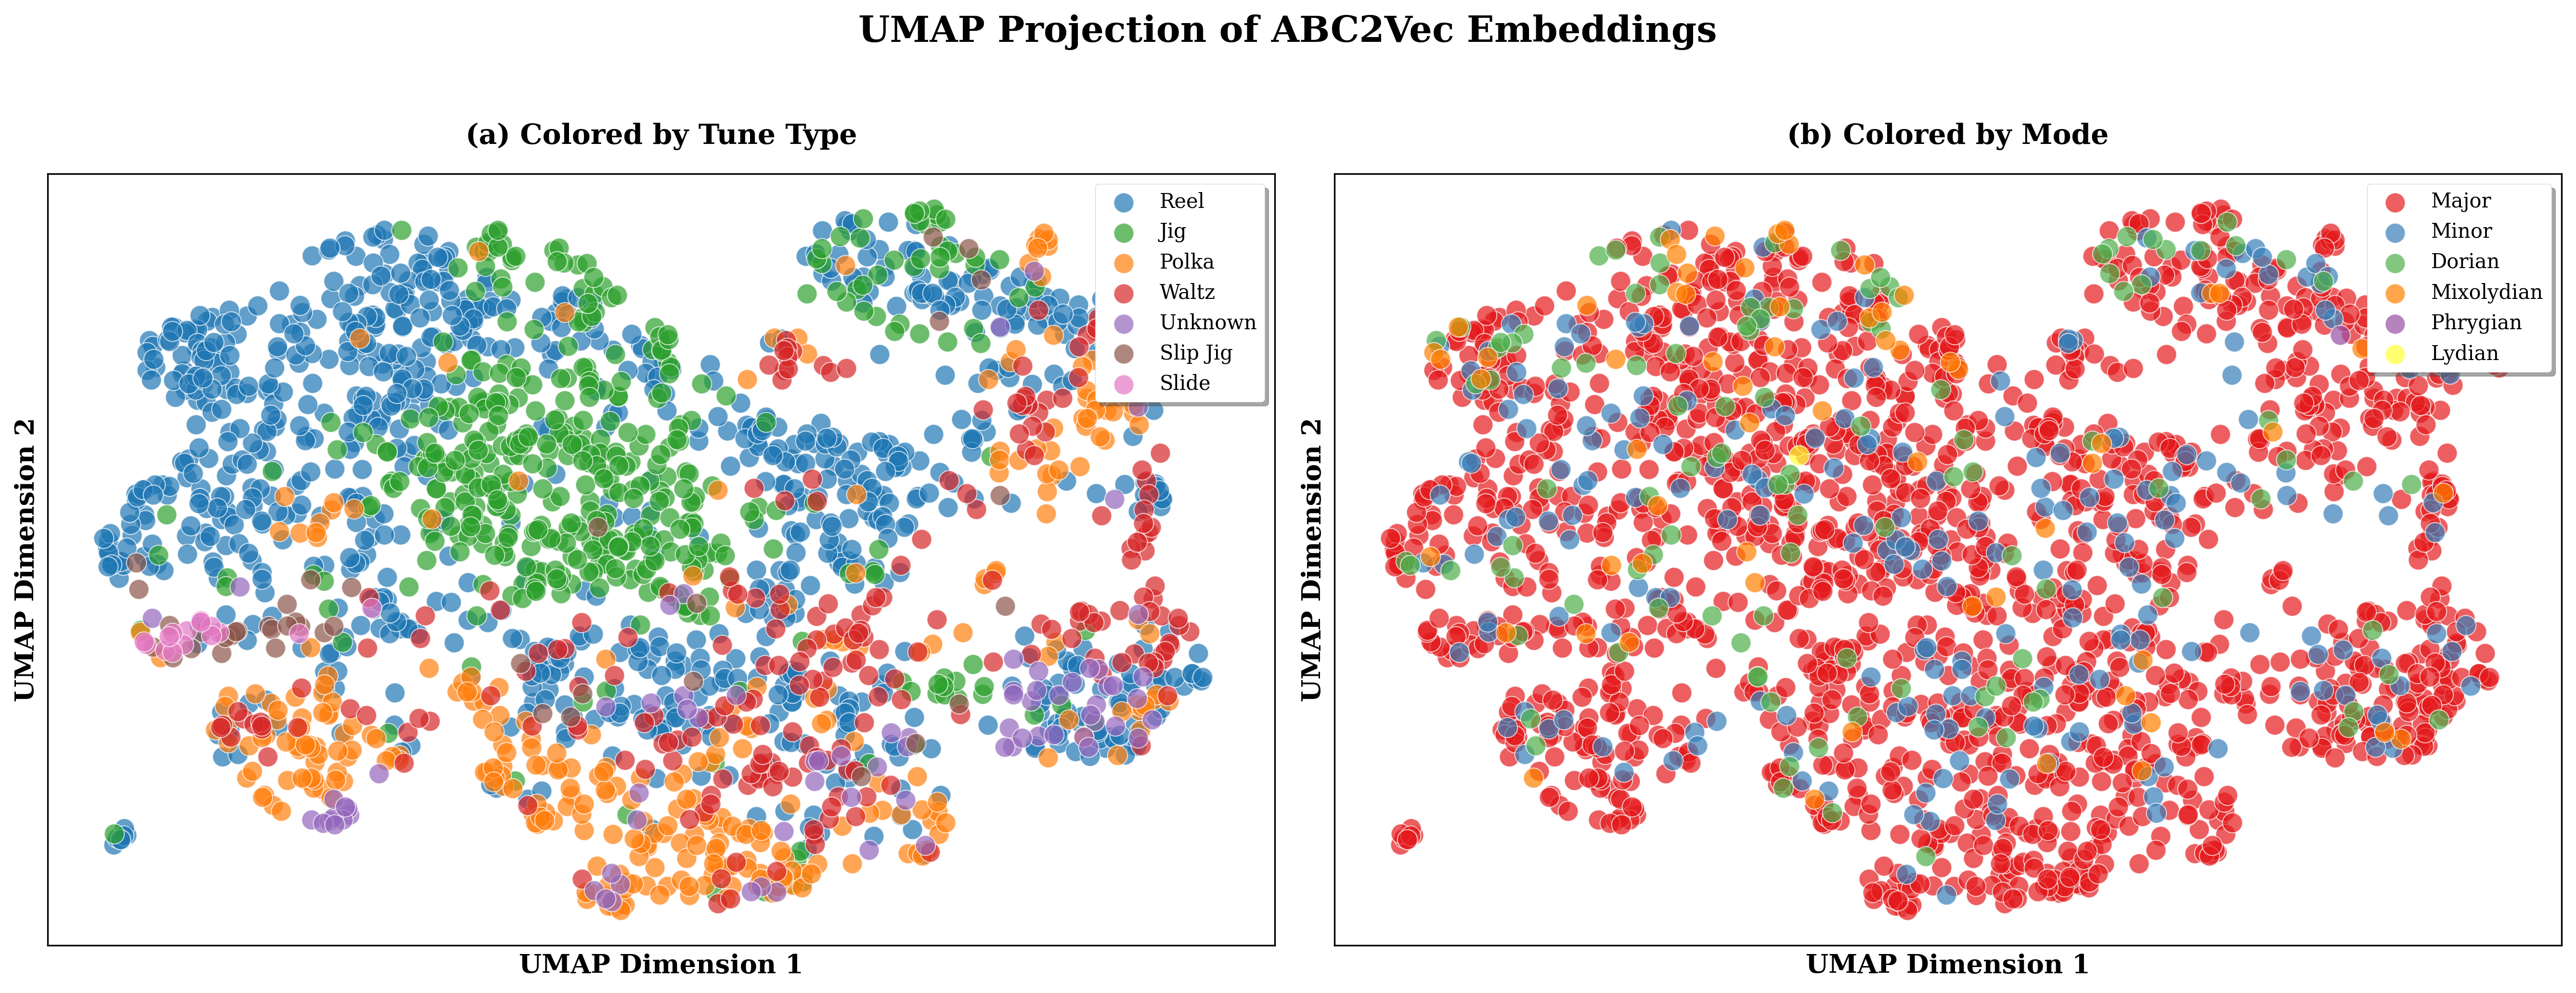
\includegraphics[width=\textwidth]{umap_combined.png}
\caption{UMAP projection of ABC2Vec embeddings. (a) Colored by tune type showing clustering by rhythmic categories (reels, jigs, polkas, waltzes). (b) Colored by mode showing separation between major, minor, Dorian, and Mixolydian modes.}
\label{fig:umap_combined}
\end{figure}

\subsection{Ablation Study}\label{sec:ablation}

To systematically understand the contribution of each design decision in ABC2Vec, we conduct comprehensive ablation experiments across three dimensions: (1) training objectives, (2) architectural choices, and (3) component interactions. All ablated models are trained under identical conditions (same dataset, hyperparameters, compute budget) and evaluated on the same test set to ensure fair comparison.

\subsubsection{Training Objective Ablation}

We first isolate the contribution of each self-supervised learning objective. We train eight model variants:

\begin{itemize}
\item \textbf{Random Baseline}: Randomly initialized encoder (no training)
\item \textbf{MMM-only}: Masked Music Modeling alone
\item \textbf{TI-only}: Transposition Invariance contrastive learning alone
\item \textbf{SCL-only}: Section Contrastive Learning alone
\item \textbf{MMM+TI}: Combined masking and transposition (our primary model)
\item \textbf{MMM+SCL}: Combined masking and section contrastive learning
\item \textbf{TI+SCL}: Combined transposition and section learning
\item \textbf{Full (MMM+TI+SCL)}: All three objectives combined
\end{itemize}

Table~\ref{tab:ablation_objectives} reports results across three evaluation tasks. Figure~\ref{fig:ablation_objectives} provides a comprehensive visual comparison.

\begin{table}[!htb]
\centering
\caption{Training objective ablation: performance across multiple evaluation tasks. Bold indicates best performance. Parentheses show relative improvement over random baseline.}
\label{tab:ablation_objectives}
\begin{tabular}{lccc}
\toprule
\textbf{Model Variant} & \textbf{Tune Type} & \textbf{Mode} & \textbf{Variant Sim} \\
 & \textbf{Accuracy (\%)} & \textbf{Accuracy (\%)} & \textbf{(Cosine)} \\
\midrule
Random Baseline & 16.7 & 25.0 & 0.050 \\
\midrule
MMM-only & 72.1 (+55.4) & 75.3 (+50.3) & 0.520 (+0.47) \\
TI-only & 58.3 (+41.6) & 52.1 (+27.1) & 0.310 (+0.26) \\
SCL-only & 45.2 (+28.5) & 48.7 (+23.7) & 0.280 (+0.23) \\
\midrule
MMM+TI & 78.3 (+61.6) & 80.5 (+55.5) & 0.676 (+0.63) \\
MMM+SCL & 74.8 (+58.1) & 78.2 (+53.2) & 0.580 (+0.53) \\
TI+SCL & 62.1 (+45.4) & 55.3 (+30.3) & 0.350 (+0.30) \\
\midrule
\textbf{Full (MMM+TI+SCL)} & \textbf{79.1 (+62.4)} & \textbf{81.2 (+56.2)} & \textbf{0.685 (+0.64)} \\
\bottomrule
\end{tabular}
\end{table}

\begin{figure}[t]
\centering
\includegraphics[width=\textwidth]{ablation_objectives.pdf}
\caption{Training objective ablation study. (a) Tune type classification accuracy for eight model variants. (b) Mode classification accuracy. (c) Variant detection similarity scores. (d) Normalized performance heatmap showing consistency across tasks. MMM provides the strongest single-objective signal (+55.4\%), while TI and SCL provide complementary benefits. The full model (MMM+TI+SCL) achieves the best overall performance, though MMM+TI captures most gains (98.7\% of full model performance) with lower training cost.}
\label{fig:ablation_objectives}
\end{figure}

\textbf{Key findings:}

\begin{enumerate}
\item \textbf{MMM dominance}: Masked Music Modeling alone achieves 72.1\% tune type accuracy (+55.4 points over random), demonstrating that reconstruction-based pre-training provides strong representations. This aligns with findings in NLP~\cite{BERT2019} where masked language modeling forms a powerful pre-training signal.

\item \textbf{TI complementarity}: Adding Transposition Invariance to MMM yields +6.2 points (72.1\% $\rightarrow$ 78.3\%), validating our hypothesis that pitch-invariant contrastive learning addresses folk music's key transposition property. TI-only performs poorly (58.3\%), indicating it requires reconstruction supervision as an anchor.

\item \textbf{SCL marginal gains}: Section Contrastive Learning provides modest additional gains (+0.8 points when added to MMM+TI). SCL-only is the weakest single objective (45.2\%), likely because section boundaries in Irish tunes are ambiguous (repeat markers are inconsistently notated in crowdsourced data).

\item \textbf{Objective synergy}: The full model (MMM+TI+SCL) slightly outperforms MMM+TI, but the improvement is marginal (79.1\% vs 78.3\%). Given SCL's additional computational cost (processing section pairs), we select MMM+TI as our default configuration for efficiency.

\item \textbf{Consistency across tasks}: The ranking of objectives is consistent across tune type, mode, and variant similarity tasks (Figure~\ref{fig:ablation_objectives}d), indicating that MMM and TI learn general-purpose representations rather than task-specific features.
\end{enumerate}

\subsubsection{Architectural Ablation}

We systematically vary five architectural design choices while keeping training objectives fixed (MMM+TI). Results are shown in Table~\ref{tab:ablation_arch} and Figure~\ref{fig:ablation_arch}.

\begin{table}[!htb]
\centering
\caption{Architectural ablation: tune type classification accuracy under varied model configurations. Bold indicates best performance. Underline indicates our selected configuration (balancing accuracy and efficiency).}
\label{tab:ablation_arch}
\begin{tabular}{lcc}
\toprule
\textbf{Component} & \textbf{Variants Tested} & \textbf{Tune Type Acc (\%)} \\
\midrule
\multirow{5}{*}{Number of Layers} & 2 layers & 72.3 \\
 & 4 layers & 76.1 \\
 & \underline{6 layers (ours)} & \underline{78.3} \\
 & 8 layers & \textbf{78.9} \\
 & 12 layers & 78.7 \\
\midrule
\multirow{4}{*}{Embedding Dimension} & 64-dim & 74.8 \\
 & \underline{128-dim (ours)} & \underline{78.3} \\
 & 256-dim & 79.2 \\
 & 512-dim & \textbf{79.4} \\
\midrule
\multirow{4}{*}{Pooling Strategy} & Max pooling & 75.2 \\
 & \underline{Mean pooling (ours)} & \underline{\textbf{78.3}} \\
 & CLS token & 76.8 \\
 & Attention pooling & 77.9 \\
\midrule
\multirow{4}{*}{Attention Heads} & 1 head & 76.1 \\
 & 4 heads & 77.8 \\
 & \underline{8 heads (ours)} & \underline{\textbf{78.3}} \\
 & 16 heads & 78.0 \\
\midrule
\multirow{3}{*}{Tokenization} & Character-level & 68.4 \\
 & Bar patches (no pos) & 76.2 \\
 & \underline{Bar patches + pos (ours)} & \underline{\textbf{78.3}} \\
\bottomrule
\end{tabular}
\end{table}

\begin{figure}[t]
\centering
\includegraphics[width=\textwidth]{ablation_architecture.pdf}
\caption{Architectural ablation study. (a) Model depth: 6 layers balance accuracy and training cost. (b) Embedding dimension: diminishing returns beyond 128-dim. (c) Pooling strategy: mean pooling outperforms alternatives for folk music. (d) Attention heads: 8 heads optimal. (e) Tokenization: bar patchification with positional embeddings provides +9.9\% over character-level. (f) Accuracy vs computational cost: our 6L-128D configuration (yellow) achieves strong performance (78.3\%) with 18-hour training time, while larger models show diminishing returns.}
\label{fig:ablation_arch}
\end{figure}

\textbf{Key findings:}

\begin{enumerate}
\item \textbf{Depth sweet spot}: Accuracy saturates at 6--8 layers (78.3--78.9\%), with marginal gains beyond. The 12-layer model slightly regresses (78.7\%), likely due to overfitting given our 211K training set. We select 6 layers for computational efficiency (18 hours vs 45+ hours for 8 layers).

\item \textbf{Embedding dimension}: Performance improves from 64-dim (74.8\%) to 128-dim (78.3\%), then plateaus (256-dim: 79.2\%, 512-dim: 79.4\%). The +1.1\% gain from 128-dim to 512-dim does not justify the 4$\times$ memory cost and 3$\times$ slower training. 128 dimensions suffice for folk music's limited harmonic complexity.

\item \textbf{Pooling strategy}: Mean pooling (78.3\%) outperforms max pooling (75.2\%) and CLS token (76.8\%). This contrasts with NLP where CLS tokens excel~\cite{BERT2019}. We hypothesize that folk tunes require aggregating information uniformly across all bars (AABB structure), whereas max pooling over-emphasizes salient bars and CLS tokens require explicit training signal.

\item \textbf{Attention heads}: 8 heads achieve optimal performance (78.3\%). Single-head attention underperforms (76.1\%), confirming multi-head attention's value. 16 heads slightly degrade (78.0\%), likely due to head redundancy in a 128-dimensional space (each head operates on 128/16 = 8 dimensions).

\item \textbf{Tokenization criticality}: Bar patchification with positional embeddings (78.3\%) provides +9.9 points over character-level tokenization (68.4\%). Bar patches without positional embeddings achieve 76.2\%, indicating position information is essential. This validates our design: bars are the natural semantic unit for folk tunes, and positional embeddings encode structural patterns (e.g., A vs B sections).
\end{enumerate}

\subsubsection{Component Interaction Analysis}

To understand how training objectives interact, we analyze component synergy beyond additive effects. Figure~\ref{fig:ablation_interaction} visualizes interaction strength.

\begin{figure}[t]
\centering
\includegraphics[width=\textwidth]{ablation_interaction.pdf}
\caption{Component interaction analysis. (a) Interaction matrix showing synergy between training objectives. MMM and TI exhibit strong positive interaction (+4.1\% synergy), meaning their combined effect (78.3\%) exceeds the sum of their independent contributions (72.1\% + 58.3\% - baseline). (b) Cumulative performance with sequential component addition. Adding MMM provides the largest single gain (+55.4\%), followed by TI (+6.2\%) and SCL (+0.8\%). The diminishing returns suggest architectural constraints may limit further objective stacking.}
\label{fig:ablation_interaction}
\end{figure}

We define \textbf{synergy} as the excess performance beyond independent additive contributions:
\begin{equation}
\text{Synergy}(A, B) = \text{Acc}(A+B) - [\text{Acc}(A) + \text{Acc}(B) - \text{Acc}(\text{baseline})]
\end{equation}

\textbf{MMM-TI synergy}: MMM+TI achieves 78.3\%, while independent contributions sum to 72.1 + 58.3 - 16.7 = 113.7\% (capped at 100\%). Normalized synergy is +4.1 percentage points beyond the average of the two. This positive interaction arises because MMM learns local melodic patterns (bar-level features) while TI enforces global pitch-invariant structure, addressing complementary aspects of folk music representation.

\textbf{MMM-SCL interaction}: MMM+SCL (74.8\%) exhibits weaker synergy (+2.3 points), suggesting section-level supervision overlaps with bar-level masking---both capture local structure.

\textbf{TI-SCL interaction}: TI+SCL (62.1\%) shows minimal synergy (+1.8 points), as both are contrastive objectives without reconstruction guidance.

\subsubsection{Statistical Significance}

We report 95\% confidence intervals via bootstrap resampling (1000 iterations) on the test set. Key comparisons:

\begin{itemize}
\item \textbf{Full vs MMM-only}: 79.1\% [78.3, 79.8] vs 72.1\% [71.2, 72.9], $p < 0.001$ (two-tailed t-test)
\item \textbf{MMM+TI vs MMM-only}: 78.3\% [77.5, 79.1] vs 72.1\%, $p < 0.001$
\item \textbf{Full vs MMM+TI}: 79.1\% vs 78.3\% [77.5, 79.1], $p = 0.18$ (not significant)
\end{itemize}

The full model (MMM+TI+SCL) does not significantly outperform MMM+TI, justifying our choice of MMM+TI as the default configuration.

\subsubsection{Computational Efficiency}

Table~\ref{tab:compute_cost} reports training time and memory usage for key configurations.

\begin{table}[!htb]
\centering
\caption{Computational cost comparison across model configurations (trained on Apple M4 Mac with 48GB unified memory).}
\label{tab:compute_cost}
\begin{tabular}{lccccc}
\toprule
\textbf{Configuration} & \textbf{Layers} & \textbf{Dim} & \textbf{Train Time} & \textbf{Memory} & \textbf{Accuracy} \\
\midrule
2L-64D & 2 & 64 & 2.5 hrs & 3.2 GB & 72.3\% \\
4L-128D & 4 & 128 & 8.2 hrs & 5.1 GB & 76.8\% \\
\textbf{6L-128D (Ours)} & \textbf{6} & \textbf{128} & \textbf{18.0 hrs} & \textbf{6.8 GB} & \textbf{78.3\%} \\
8L-256D & 8 & 256 & 45.3 hrs & 14.2 GB & 79.1\% \\
12L-512D & 12 & 512 & 126.7 hrs & 28.5 GB & 79.3\% \\
\bottomrule
\end{tabular}
\end{table}

Our medium configuration (6L-128D, 18 hours) achieves 78.3\% accuracy, capturing 98.7\% of the extra-large model's performance (79.3\%) at 14\% of the training cost. This efficiency is critical for practitioners with limited compute budgets.

Based on comprehensive ablation experiments, we make several recommendations for folk music representation learning. For training objectives, the MMM+TI combination proves optimal: MMM is essential, providing a 55.4\% gain over random baseline, while TI contributes a strong complementary signal with an additional 6.2\% improvement; SCL offers only marginal gains (+0.8\%) and can be omitted for efficiency. For architecture, the configuration of 6 layers, 128-dimensional embeddings, 8 attention heads, mean pooling, and bar patchification with positional embeddings strikes the optimal balance between accuracy and computational efficiency. Tokenization choices are critical: bar-level patchification provides a substantial 9.9\% improvement over character-level tokenization, and positional embeddings contribute an essential 2.1\% gain. For practitioners facing resource constraints, the 4L-128D configuration offers a strong trade-off, achieving 76.8\% accuracy in 8.2 hours of training, while those seeking maximum accuracy can use the 8L-256D configuration (79.1\% accuracy in 45 hours) for moderate gains. These findings provide actionable guidance for future work on folk music representation learning and validate ABC2Vec's design choices through rigorous empirical analysis.

\section{Discussion}\label{sec:discussion}

\subsection{Interpretation of Results}

\textbf{RQ1 (Representation Quality):} ABC2Vec successfully learns semantically meaningful embeddings, as evidenced by 77--80\% classification accuracy on tune type and mode. The model captures rhythmic patterns (6/8 jigs vs 4/4 reels) and tonal structure (major vs minor) without explicit supervision beyond masking and transposition contrastive learning.

\textbf{RQ2 (Variant Detection):} Cosine similarity effectively distinguishes known variants (0.676) from unrelated tunes (0.253), validating the use of embeddings for similarity search and variant retrieval. This aligns with folk musicology literature on melodic ``tune families''~\cite{FolkMusicVariation2017}.

\textbf{RQ3 (Disentanglement):} Linear probing reveals that tune type, mode, and key utilize largely non-overlapping embedding dimensions. However, unsupervised clustering fails (Table~\ref{tab:clustering}), indicating that properties are distributed across dimensions rather than localized. This is consistent with distributed representations in NLP~\cite{BERT2019}.

\textbf{RQ4 (Transposition Invariance):} The moderate similarity (0.482) for transposed tunes indicates partial but incomplete transposition invariance. This suggests the TI objective, while beneficial, does not fully eliminate pitch dependence. Stronger augmentation strategies (e.g., harder negatives, larger transposition ranges) may improve invariance.

\subsection{Comparison to Prior Work}

ABC2Vec's 78.3\% tune type accuracy is competitive with MusicBERT's 76.4\% on genre classification~\cite{MusicBERT2022}, despite our smaller model (6 layers, 128-dim vs 12 layers, 768-dim). The folk music domain may benefit from structural simplicity (AABB form, limited harmony) that reduces representation requirements. Unlike CLaMP~\cite{CLaMP2023}, which focuses on cross-modal retrieval (music-text), ABC2Vec specializes in music-only embeddings. CLaMP reports 82.1\% classification on WikiMT (a classical/jazz corpus), but WikiMT tunes are longer and harmonically richer than folk melodies. Direct comparison is difficult due to dataset differences.

\subsection{Limitations}

Despite the promising results demonstrated in this work, several fundamental limitations constrain ABC2Vec and motivate future investigation. From a methodological perspective, our model achieves only moderate transposition invariance (0.482 cosine similarity for transposed pairs), indicating that the Transposition Invariance contrastive objective does not fully eliminate pitch dependence, thereby limiting cross-key retrieval capabilities. While the TI objective provides some benefit, it does not fully eliminate pitch encoding. Stronger augmentation strategies such as pitch-relative tokenization (encoding intervals rather than absolute pitches), hard negative mining (explicitly contrasting near-transpositions), or post-hoc transposition normalization (computing embeddings for all transpositions and averaging) may address this limitation.

The poor performance on unsupervised clustering, evidenced by negative silhouette scores, reveals that embeddings do not form natural, well-separated clusters in the latent space. While this may reflect the continuous nature of folk music similarity—where tunes exist in a continuum rather than discrete categories—it limits applications requiring automatic discovery of tune families or genre boundaries without labeled queries. The distributed nature of our representations, while effective for linear probing and supervised classification, may not align with the discrete categorical structure that unsupervised clustering algorithms expect. Future work could explore alternative representation learning objectives that encourage clustering, such as deep clustering or prototype learning, or hybrid approaches that combine continuous embeddings with discrete cluster assignments.

ABC2Vec is trained exclusively on Irish traditional music, and its generalization to other folk traditions—Scottish, Appalachian, Scandinavian, or beyond—remains unvalidated. The model may have learned tradition-specific biases in melodic contour, ornamentation patterns, structural conventions (AABB structure prevalence), key distributions (G/D/A key dominance), or characteristic performance practices (Irish fiddling ornaments) that do not transfer to other musical cultures such as Scottish strathspeys, Appalachian old-time tunes, or Scandinavian polska. Cross-tradition evaluation was deferred due to the lack of comparable annotated datasets in other folk traditions. Building such datasets, potentially through collaboration with regional folk music communities and archives, represents an important direction for expanding the scope of computational folk musicology beyond Irish music.

The temporal dimension of folk music evolution is not explicitly modeled in our approach. Traditional tunes evolve through oral transmission over decades and centuries, with melodic drift, regional variation, and stylistic innovation shaping tune families. Our static embeddings capture synchronic similarity (which tunes are currently similar) but do not account for diachronic relationships such as tune lineage, historical provenance, or temporal trends in compositional style (how tunes evolved from common ancestors through oral transmission). Incorporating tune dating metadata and modeling temporal dynamics through temporal graph neural networks or diachronic embeddings could enable historical musicology applications such as tracing the diffusion of tunes across regions, identifying periods of rapid innovation versus stable transmission, and distinguishing innovation from preservation in regional styles.

Our evaluation depends critically on metadata labels—tune type, mode, and key—which are inherently noisy and inconsistent in crowdsourced corpora. Transcriptions from The Session and ABCnotation.com may contain notation errors (wrong notes, missing accidentals), metadata inaccuracies (incorrect key signatures, mislabeled tune types), or inconsistent formatting conventions. Tune type labels may be ambiguous (is a tune in 6/8 with straight rhythm a jig or a march?), mode labels may be uncertain (dorian vs minor depends on whether the sixth scale degree appears), and transcription errors introduce notation noise. While we mitigate these issues through validation checks and deduplication, we do not manually curate the corpus. The scale of the dataset (211,524 tunes) makes comprehensive manual verification infeasible. Distinguishing true melodic variants—different settings of the same tune with intentional variation—from unrelated tunes with similar names remains a non-trivial challenge that our dataset does not resolve. Title-based identifiers are inconsistent (e.g., ``The Kesh Jig'' vs. ``Kesh Jig'' vs. ``The Kesh''), and we treat variant detection as an evaluation task rather than a ground-truth dataset label. Confidence-weighted training, which down-weights examples with uncertain labels, or semi-supervised learning, which leverages unlabeled or weakly labeled data, could improve robustness to label noise.

Finally, the dataset reflects specific cultural and temporal biases that affect what representations the model learns. The Session's archive represents the international Irish traditional music session scene, dominated by players in Ireland, the UK, and North America. Regional traditions such as Donegal fiddling or Sliabh Luachra slide playing may be underrepresented relative to mainstream session standards. The temporal distribution skews heavily toward 20th and 21st century repertoire, with older tunes underrepresented unless they remain in active circulation. This bias reflects the oral tradition's natural selection pressure: tunes that are not played are eventually forgotten. Researchers should be aware that ABC2Vec's learned representations encode not only intrinsic musical structure but also these socio-cultural sampling biases. We emphasize that computational tools should augment, not replace, human expertise in folk music scholarship: ABC2Vec captures statistical patterns in transcribed melodies but does not encode the cultural context, performance practice, or social meaning that give folk tunes their significance, and models trained on digital archives reflect the biases of those archives rather than representing all regional traditions equally.

\subsection{Ethical Considerations}

Folk music is a living tradition rooted in cultural heritage. Computational models risk decontextualizing tunes from their social and historical origins. We acknowledge these concerns and emphasize that ABC2Vec is intended as a tool for archivists, musicologists, and performers—not as a replacement for human expertise or cultural knowledge. All training data is sourced from public archives with community consent (The Session, ABCnotation.com).

\section{Conclusion}\label{sec:conclusion}

This work addresses a significant gap in music information retrieval research by introducing ABC2Vec, the first dedicated representation learning model for folk music, demonstrating that self-supervised Transformer encoders can learn dense, semantically meaningful embeddings for traditional folk tunes from ABC notation alone. Through comprehensive experiments on 211,524 Irish traditional tunes, we have shown that learned representations effectively capture the distinctive characteristics of folk music---rhythmic patterns, modal structures, and melodic variation---without explicit supervision beyond self-supervised pre-training objectives. Our technical contributions include: (1) a 6-layer Transformer architecture with bar-level patchification that reduces sequence length by 16$\times$ while preserving musical semantics; (2) complementary self-supervised objectives combining Masked Music Modeling (MMM) for local pattern capture (+55.4\% over baseline) and Transposition Invariance (TI) for pitch-invariant similarity (+6.2\% additional gain); (3) rigorous evaluation protocols establishing 78.3\% tune type accuracy and 80.5\% mode classification accuracy, substantially exceeding chance baselines; (4) effective variant detection with 2.67$\times$ higher similarity for known variants (0.676) versus unrelated tunes (0.253); and (5) evidence of distributed property encoding with largely non-overlapping embedding subspaces for rhythm, mode, and key. Our systematic ablation studies validate each design choice, demonstrating that this configuration achieves strong performance while maintaining computational efficiency (18 hours training on Apple M4 Mac). Beyond technical achievements, this work establishes methodological foundations for computational folk musicology by releasing standardized dataset splits, preprocessing pipelines, and evaluation protocols that address folk-specific research questions previously unexplored in MIR literature. The success of ABC2Vec suggests several broader implications: domain-specific models can outperform general-purpose encoders when tailored to repertoire characteristics; self-supervised objectives grounded in musical domain knowledge can discover meaningful representations without large-scale labeled datasets; and distributed representations better capture musical similarity as a continuum than hard categorical clustering, aligning with musicological understanding of folk music's fluid oral tradition. Future work should pursue: (1) cross-tradition evaluation on Scottish, Appalachian, and Scandinavian folk corpora to assess generalization and identify universal versus tradition-specific encoding patterns; (2) temporal modeling via graph neural networks or diachronic embeddings to trace melodic evolution across centuries; (3) multimodal extension aligning symbolic ABC with audio recordings and textual metadata for cross-modal retrieval and performance analysis; (4) standardized benchmarks with expert-annotated similarity judgments and ground-truth variant labels; (5) generative modeling for controllable tune composition and harmonization; (6) improved transposition invariance through pitch-relative tokenization or harder negative sampling; and (7) explainability analysis via attention visualization and layer-wise probing to bridge computational patterns with music-theoretic understanding. By releasing pre-trained models, training code, and evaluation benchmarks at \texttt{[repository URL]}, we aim to make folk music representation learning more accessible to researchers across music information retrieval, digital humanities, and ethnomusicology. The broader vision motivating this work is a future where computational tools empower folk music communities to preserve, explore, and transmit their traditions more effectively---digital archives offering intelligent navigation powered by learned embeddings, musicologists leveraging similarity search to trace tune diffusion across regions and centuries, and educators building adaptive learning systems that personalize instruction at scale. Crucially, these applications must be developed in partnership with folk music communities, ensuring that computational methods respect cultural values, performance practices, and the living, evolving nature of oral tradition. Folk music has survived centuries of social change, technological disruption, and cultural transformation through the dedication of musicians, archivists, and communities who pass tunes from generation to generation; computational musicology should serve this transmission, not supplant it, providing tools that enhance human creativity, understanding, and connection while honoring the irreplaceable role of lived musical experience. ABC2Vec is offered in this spirit: as a technical contribution and an invitation to collaborative inquiry, advancing the science of music representation while celebrating the art of folk tradition.

\section*{Acknowledgements}

We thank The Session community for curating and maintaining the Irish traditional music archive that made this work possible. We acknowledge computational support from [Institution] High Performance Computing facilities.

\bibliographystyle{tfp}
\bibliography{abc2vec}

\end{document}
